We have discussed the problem statement and motivation in the previous chapter. In order to solve the problem stated in Chapter \ref{chap:1}, we have implemented a solution based on the machine learning approach. A clear understanding of concepts and terminologies of machine learning is required for the next chapters. Moreover, there are many different terms for a same concept in the areas of Data Science and Machine Learning which can be used interchangeably. Since later chapters will make heavy use of these jargons it is necessary to establish a common base vocabulary to avoid confusion for the readers. So in this chapter we will explain Machine Learning and Scene Classification exhaustively. We will also discuss different computer vision tasks and how a neural network works.

% Image classification, Semantic Segmentation, Classification + localization, Object detection, , Instance segmentation.

% Machine learning and AI are frequently used as interchangeable terms. However, they are slightly different aspects of the same concept. In fact, AI is the parent to machine learning. https://towardsdatascience.com/artificial-intelligence-vs-machine-learning-a7d7a13b72d8


% In the previous chapter, we discussed the problem statement, motivation, and goals of this thesis. Again, in this thesis, we are trying to build an intelligent system that can classify the documents (tax-related) efficiently. I also mentioned that to solve this problem, we implemented different solutions but since our major solution is based on machine learning techniques, so we will mostly talk about that method. In the next few chapters, we will see and discuss the technologies and methodologies used to implement the solutions and how we trained a machine learning model for document classification but to understand these things, one need to have some pre-requisite knowledge in the domain of machine learning. So, in this chapter, we will explain the machine learning in detail. Along with that, we will also shed the light on core concepts of Artificial Neural Networks and Convolutional Neural Networks as it is a major part of the proposed solution.

\section{Artificial Intelligence and Machine Learning}
Artificial Intelligence and Machine Learning are often used together and in recent years has gained great popularity. Artificial Intelligence or AI is a broad area in Computer Science which mimics human intelligence. It focuses on theory and development of intelligent computer systems that can do activities like speech recognition, visual perception, decision-making, learning, planning, etc. AI systems need a large dataset to train its model and faster hardware to process the data. Artificial Intelligence has made significant advances in the past few years because of abundance of data through internet and cheap sensors and spectacular improvements in hardware capabilities.
\par
Machine learning is a specific subset of AI that trains a machine how to learn and improve from experience without being explicitly programmed. Machine learning is increasingly ubiquitous in consumer products such as smartphones, cheap sensors and IoT devices. Most of the people are using it in one way or another and without even knowing. Machine learning is changing our everyday life and powers so many aspects of our modern society. Some if it's applications are: search engine results refinement, spam/content filtering on social networks, Virtual Personal Assistants (like Siri, Alexa, Google Now), recommendations on e-commerce web-applications, online fraud detection, video surveillance, online customer support, and so on.

\par
Artificial Intelligence and machine learning is constantly pushing the boundaries of what machines are capable of and even in some intellectual areas where these systems are already performing better than humans. There is a lot of research going on in these fields. Researchers are proposing new applications and also optimizing existing models and algorithms.

\par
In machine learning, a model is trained by using some machine learning algorithms with a substantial amount of data to make predictions. There are a lot of different algorithms that work best for solving different problems, so we must have a good understanding of the algorithm to train our model before using it. Further sections aims to provide a rigourous, yet easy-to-follow, introduction of the main underlying concepts of machine learning, it's types and architecture.

% The recent era has witnessed many revolutionary wonders in the world of machine learning. By embracing the significance and power of it, the tech-communities around the globe are actively working on it and continuously striving to find the new horizons and possibilities in different domains to make things intelligent by leveraging the power of machine learning. According to the research, there are some tasks where machine learning has outperformed humans. The common applications of machine learning are mostly related to forecasting, classification, intelligent systems like voice assistants, etc. Furthermore, many commercial sectors are moving towards machine learning to automate their manual tasks and making their processes or systems intelligent. For example, banking sectors are using machine learning for fraud detection, in the health industry they are using it for disease diagnosis or forecasting, in online shopping portals, they are using it for showing items relevant to the user's interest. These are some of the few examples where different organizations are using machine learning to make their systems smart and independent and also to give users a better experience. 

% \par
% In machine learning, we train our model by using some machine learning algorithms with a huge amount of data to finally make predictions. There are a lot of algorithms that work best in different kinds of problems, so we need to have a better understanding of it before using any algorithm. Taking these things into account, further sections will explain the concepts of machine learning, it's types and architecture in detail.

\section{Definitions of Machine Learning}
Machine learning is a broad study and different researchers have given rather different definitions of it. Some of the definitions from renouned sources are mentioned below:
\newline
\newline
\par
\q{Machine learning research is part of research on artificial intelligence, seeking to provide knowledge to computers through data, observations and interacting with the world. That acquired knowledge allows computers to correctly generalize to new settings.}\cite{ml_def} By Dr. Yoshua Bengio, also known as the godfather of Artificial Intelligence
\newline
\newline
\par
\q{Machine learning is the science of getting computers to act without being explicitly programmed.} \cite{ml_def_stanford} By Stanford University
\newline
\newline
\par
\q{The field of Machine Learning seeks to answer the question: How can we build computer systems that automatically improve with experience, and what are the fundamental laws that govern all learning processes?}\cite{ml_def_cm} By Carnegie Mellon University
\newline
\newline
\par
\q{Machine Learning at its most basic is the practice of using algorithms to parse data, learn from it, and then make a determination or prediction about something in the world.}\cite{ml_def_nvidia} By Nvidia
\newline
\newline
\par
\q{Machine learning is based on algorithms that can learn from data without relying on rules-based programming.}\cite{ml_def_mckinsey} By McKinsey \& Co.

% \section{History of Machine Learning}
\section{Evolution of Machine Learning}
Just around five decades ago, machine learning was still the science fiction stuff. But today it has become basic part of our everyday life. Computer scientists, researchers, mathematicians, thinkers and philosophers had put tremendous efforts for many years in this field to come at this stage. Without that we would not have been enjoying quick web search results, self-driving cars, and intelligent voice assistants. We will try to present a overview of when and how this domain originated and developed over the years in this section.
\newline
\par
The basic concepts of machine learning largely rely on statistics and mathematics. Some of the mathematical and statistical theories like the "Least Squares method for data fitting" by Adrien-Marie Legendre in 1805 and "Bayes' Theorem" by Thomas Bayes and Pierre-Simon Laplace" in 1812 and Andrey Markov described analysis techniques later called Markov Chains in 1913 \cite{ml_history} became the foundation of modern machine learning techniques.
\newline
\begin{itemize}
  \item \textbf{1950 — Turing Test:} An English mathematician, computer scientist and cryptanalyst Alan Turing published Computing Machinery and Intelligence\cite{imitation_game}, in which he devised a hypothetical test which can determine whether a machine is capable of thinking like a human being or not. This test is famously known as 'Turing Test' named after him. The test has three parties, an interrogator, a machine, and a human. The interrogator is in a room seperated from the other human and the machine. The job of the interrogator is to try to figure out which one is the machine and which is the human by asking questions. The objective of the machine is to imitate a human being and try to justify to the interrogator to mistakenly conclude that the machine is the other human. If the interrogator is unable to distinguish the machine from the human, then it means the machine is intelligent.

  \item  \textbf{1952 — First Computer Learning Program:} In 1952, Arthur Samuel wrote the first computer learning program \cite{checkers_game}. The program was the game of checkers that can be plalyed by the person who wrote the program. It improved at the game the more it played by learning which moves lead to winning strategies and which moves to avoid within a specific scenario. This experiment verified that machine learning can be used at different situations.

  \item  \textbf{1957 — First Neural Network:} As computers became more sophisticated in the 1950's, it was finally possible to simulate a hypothetical neural network. Frank Rosenblatt, an American psychologist, designed Perceptron in 1957. It is an electronic device which showed ability to learn and was designed to predict shape and pattern recognition by imitating human brain. Then in 1960, Bernard Widrow and Marcian Hoff\cite{madaline} of Stanford University developed models they called ADALINE and MADALINE. These models were named for their use of Multiple ADAptive LINear Elements. ADALINE was able to identify binary patterns from a stream of bits and can tell what can be the next bit, while, MADALINE (Many ADALINE) was able to eliminate the echoes on phone lines. This neural network is still in commercial use.

  \item  \textbf{1990's — Data-driven approach:} Research on machine learning changed form a knowledge-driven approach to a data-driven approach. Scientists proposed new models and created programs for computers to analyze large amounts of data and draw predictions — or “learn” — from the results. In 1997, IBM's Deep Blue beats the world chess champion\cite{deepmind_chess}, largely relying on it's brute compouting power and special purpose 'chess chips'. It learned from thousands of old chess games to determine the moves to checkmate.
  
  \item  \textbf{21st Century — The boom of Machine Learning:} In 21st Century, world's technology giants like Google, Microsoft, Amazon, Intel, etc. have started to invest in artifical intelligence and machine learning to create better products and services for users. In March 2017, Google announced to change it's strategy from 'Mobile first' to 'AI first'. After one month, Microsft also announced the same. Google also announced a Tensor Processing Unit (TPU) — a specialized chips for optimizing machine learning. A lot of machine learning frameworks, libraries and tools have also been developed, like Tensorflow from Google, PyTorch, Keras, Caffe, Theano, Scikit-learn, etc. Some of the prominent projects and models includes: GoogleBrain (2012) \cite{googlebrain}, AlexNet (2012) \cite{alexnet}, DeepFace (2014) \cite{deepface}, DeepMind (2014) \cite{deepmind}, VGG16 and VGG19  (2014) \cite{vgg_19}, OpenAI (2015) \cite{openai}, ResNet (2015) \cite{resnet} and U-net (2015) \cite{unet}.
\end{itemize}

\section{Concept of Machine Learning}
In this section, we will dive into underlying concepts of machine learning which makes a system intelligent. As mentioned in the previous chapter, machine learning is a subset of artificial intelligence and that it allows computer systems the ability to automatically learn and improve from experience without being explicitly programmed, instead of programming by hand. It makes use of different algorithms and large amount of appropriate data to do this. After getting trained or running the algorithm, a machine learning system is then able to perform an intelligent task like making prediction or classification. Some of the commonly used algorithms are Linear regression, Logistic regression, Naive Bayes, K-Nearest Neighbour (kNN), Random forest, K-Means, Decision Tree, Support Vector Machine (SVM), Convolutional Neural Network, etc. A machine learning engineer or data scientist should have high-level understanding of various machine learning algorithms before selecting an algorithm to solve the problem at hand. It is because of the fact that an algorithm works best to solve a particular problem or particular set of problems. Like K-means is suitable for cluster analysis and Convolutional Neural Network (CNN) is preferred for image classification, object detection, or image segmentation. After choosing an algorithm, we need to provide the algorithm a huge amount of training data to learn from. The algorithm finds pattern in the training data and and the output is called a machine learning model. This model then can be used to make predictions.

For example, if we are solving a image classification problem like classifying photos as either containing a dog or cat, we must need to provide a lot images belonging to dogs and cats to a machine learning algorithm like (CNN). After training, the resultant model will be able identify between dogs and cat to a certain extent. There are various factors that affect the performance and correctness of the model like data quantity, data quality, feature selection, etc. Since, the model is trained on images of dogs and cats, it will not be able to classify other animals. But a questions arises here is that how machine learning approach differentiates from conventional programming approach.

\begin{figure}[H]
\centering
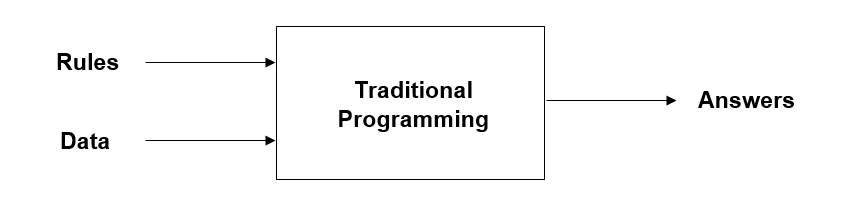
\includegraphics[scale=0.7]{images/Chapter2/TP.PNG}
\caption{Conventional Programming model}
\label{tp-model}
\end{figure}
\par

Conventional programming, as you can see in the Figure \ref{tp-model}, the first task is the creation of the most suitable algorithm and writing the code or rules for a defined set of scenarios. Then, input or data is to be provided and if the algorithm is correct we get the expected results.

% For example, if you want to create a program that should calculate employee's annual salary then you have to implement the entire logic of the program like from where the employee salary should fetch, what are the values that needs to be consider for calculation and also need to define the input parameters like employee id or name, year of salary calculation, etc. It means that this program is not independent and cannot run on its own unless these things have defined by someone.


\begin{figure}[H]
  \centering
  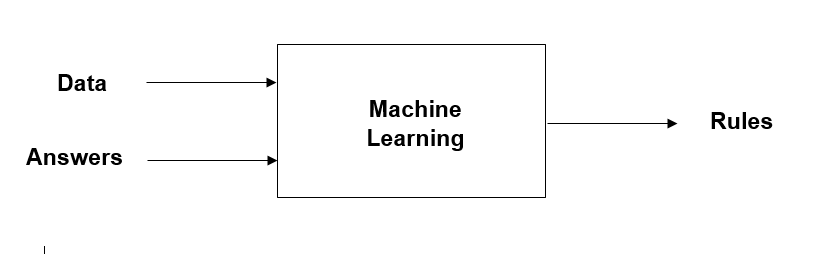
\includegraphics[scale=0.7]{images/Chapter2/ML.PNG}
  \caption{Machine Learning model}
  \label{mlp-model}
\end{figure}
\par
Machine learning just like Artificial intelligence is not a substitution, but supplementation for conventional programming approaches. In machine learning, the inputs to the systems are data and labels/answers and the choosen algorithm automatically formulates the rules from the data. We will use the term \q{prediction} for the rules generated from now on.

% On the other hand, in machine learning, the inputs to the systems are data and answers and the result are rules. It means that to develop a machine learning program, we have to feed the program a lot of data as an input and at the same time we also have to tell the output or answers of these inputs. Based on these two things, the systems analyze the data and it's result and tries to learn automatically the rules to generate the result as output. Here, it should be noted that we are not implementing any kind of logic as we were doing in the conventional programming to generate the result explicitly but here the system learns or create that logic by itself which is actually the main feature of machine learning and in the end based on the learning from data and their answers, it will be able to perform further calculations or tasks by itself independently. We saw how machine learning is different and more powerful than conventional programming. We also tried to explain the basic concept behind machine learning which is that the dependency of the output heavily relies on the data and its output which we often call labels or tags in it.
% \section{Training Machine Learning Model}
% Machine learning have many active research areas. Researchers and machine learning engineers have been presenting their own model for the problem at hand. However, the underlying concepts and method of training a model remains same. In this section, we will discuss the process of training a model using a comprehensive figure below.

% \begin{figure}[H]
% \centering
% 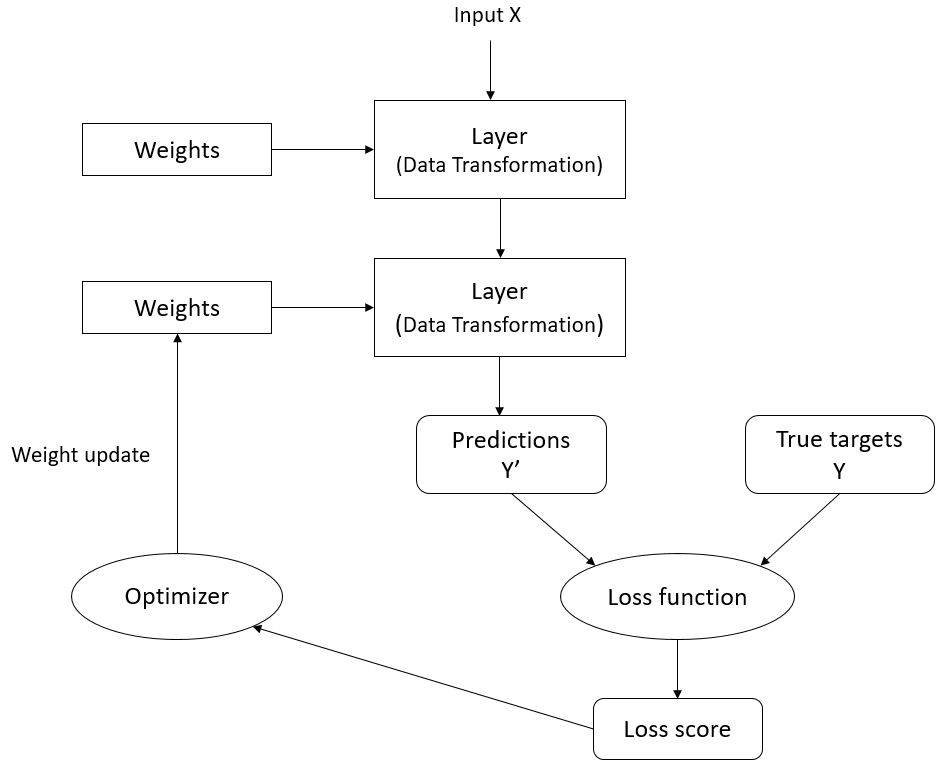
\includegraphics[scale=0.7]{images/Chapter2/ml-training-arch.png}
% \caption{Machine Learning training architecture}
% \label{mlt-arch}
% \end{figure}
% \par
% Training a model consists of a complete cycle with different phases. Consider the above Figure \ref{mlt-arch} as a training architecture of a machine learning model. Let X is our training data for our model, the first step is to pass training data X to the Layers. Here, both the layers are considered as a machine learning model. In these layers, we can increase or decrease the layers of our model as per our requirement. In these layers, data is transformed into different forms. The purpose of this transformation is to make learning easier and efficient for our model. The technique for data transformation for the model varies with the different solutions as each one implements the solution according to their business model. Each layer in the model learns from the data and store particular information about it. During the training phase, the data passed to the model breaks into two parts, training and testing which is done to check the performance of the model. After processing all the input data by the model, now the prediction phase starts, and the model starts the prediction Y' on each input data. After all the predictions, the results Y' along with the true targets Y, which are the correct labeled pre-assigned to the data, passed to the loss function. In the \q{loss function}, we evaluate how well our training algorithm modeling the input dataset. If the predictions are not as expected, then it gives a higher number. If the predictions are good and as expected, then the output will be a smaller number. This output is in the form of a number and is called \q{loss value} which indicates whether our model is well trained for the given dataset or not. If the loss value is within the threshold then our model is fine and good to go but in case the loss value is very high, then there are some additional steps need to perform to minimize the loss value. In the case of higher loss values, we optimize or tune our weights for the model. Here, weights are the numerical value which are the parameters set for our model. The method of fine-tuning the weights are random and we need to keep hit and try until the satisfactory results are achieved. After optimizing weights, the same process starts again, to train the model with new weights on the given data X and then make predictions Y' and calculate the loss value with the help of loss function.
\section{Machine Learning Pipeline/Workflow}
% In the last section, we discussed the underlying concepts and machine learning approach.
This section focuses on the important steps that are involved in a machine learning project which will help in explaining our implementation for this project. We will also discuss each step briefly and their order as well. A comprehensive figure of the whole process can be found below for reference:

% In the previous section, we discussed the cycle of how to train a machine learning model. This section is kind of more generalize and here we will discuss that what is the starting point of the project, what are the essential phases involved to work on a full-fledged machine learning project, what is the sequence of these phases and the complete lifecycle this project. For this purpose and the sake of clarity, we will take the reference of the below figure to explain the whole process:
\begin{figure}[H]
\centering
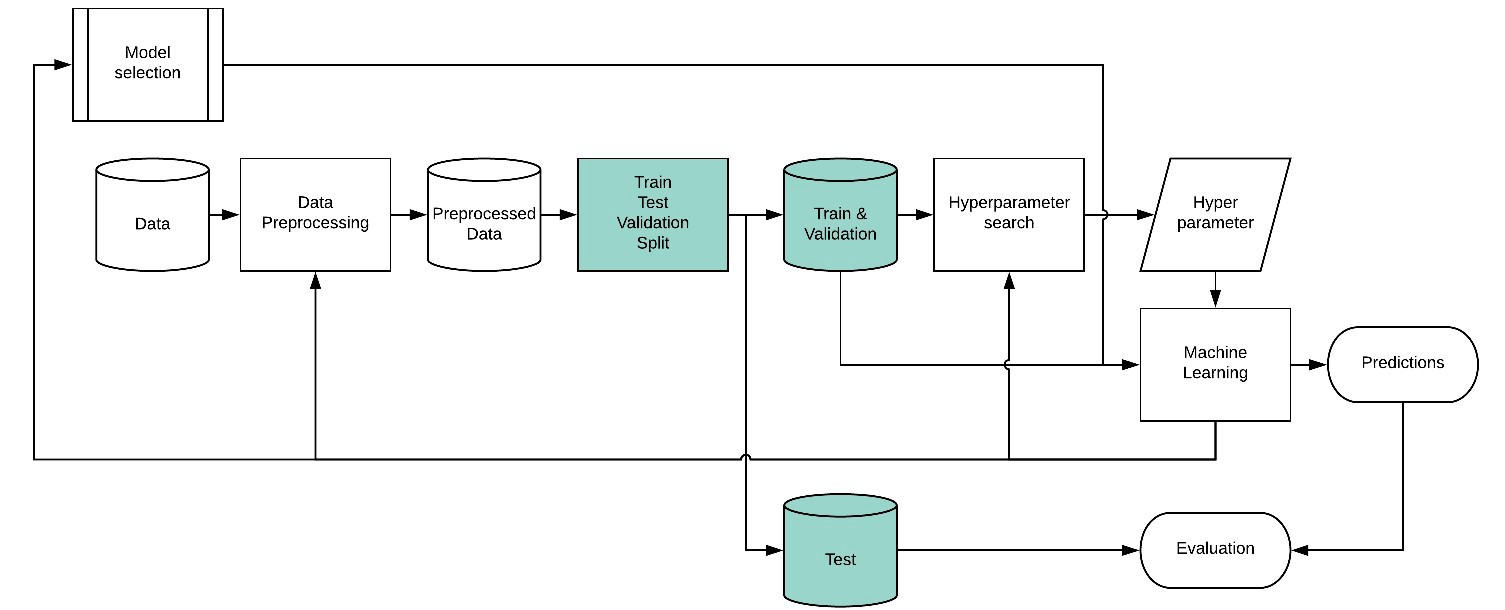
\includegraphics[scale=0.3]{images/Chapter2/ml-pipeline.jpg}
\caption{Machine Learning Workflow \cite{ml-pipeline}}
\label{ml-pipeline}
\end{figure}
\par
The sequence of the processes or the workflow in the figure above \ref{ml-pipeline} is simple but there are few steps from where we can go back to a previous step to fine-tune or change a process or parameter. The main processes are mentioned below:
\newline
\begin{enumerate}
  \item  Data Acquisition
  \item  Data Pre-Processing
  \item  Data Splitting
  \item  Model Selection
  \item  Model Training
  \item  Model Evaluation
  \item  Fine-Tuning Hyperparameters
  \item  Predictions
\end{enumerate}
\par
The first and foremost step is to have a clear understanding of the problem. and is better to have a problem statement. Only after analyzing the problem we should move forward. As we mentioned before a machine learning model requires data and as shown in the figure \ref{ml-pipeline} the starting processes are associated to data, which include \q{data acquisition}, \q{data pre-processing} and \q{data splitting}. The quality and quantity of labeled data are very crucial for improving the predictive power of a ML algorithm. Data can be in at various sources and in different formats, so the first step is to \q{acquire data}. But the collected data cannot be used directly for performing the analysis process as there might be a lot of missing data, noisy data, irrelevant and redundant data, extremely large values, or in raw format. Therefore, we need to detect and correct corrupt or inaccurate data by modifying, replacing or removing it. This process is known as \q{Data Pre-processing} or \q{Data Cleaning} or \q{Data Preparation}. Data pre-processing is one of the most important steps in machine learning. It is the most important step that helps in building machine learning models more accurately. In machine learning, there is a 80/20 rule. Most scientists or ML engineers spend 80\% of their time finding, cleaning, and reorganizing and 20\% of their time on actual data analysis. After that, the process of \q{Data splitting} usually split into training data, test data and validation data. Training portion of the data is used to develop a predictive model, the testing data to evaluate the model's performance and validation data to give an estimate of model skill while fine-tuning model's hyperparameters.
\newline
\par
\q{Model Selection} is the process of combining data and prior information to choose among a group of machine learning models. It's the step where the domain knowledge helps the implementor to choose the most suitable model for the problem at hand. Then the process of \q{training} the selected machine learning model starts with the processed/cleaned data. Model training start with set of default hyperparameters which optimizes while the training process. The method of optimizing or fine-tuning the paramters are random and we need to keep hit and try until the satisfactory results are achieved. We repeat the same process of optimizing the parameters to train the model with new parameters on the given data until desired performance, which is measured using validation data, is achieved. In the last step, of \q{Model Evalaution} the performance or the accuracy of the model is evaluated using the test data.
% \newline
% \par
% At the end of the model evaluation phase, there can be two scenarios, either the model is working fine which is quite ideal and unrealistic at the same time, in this case, our model is fine and good to go for future predictions. Another scenario is that our model is not predicting as expected and needs to be modified. From this stage, we can revert to multiple stages as if the results are totally off then maybe we are not using the suitable model and need to try other models. Other than that, if the results are a bit unexpected then we can tune the hyperparameter metrics and train our model again with new parameters or also check the data if there is any error or missing data and remove it. This phase is called \q{Fine-tuning Hyperparameters}. In this phase, we will keep hitting and try out these things until we have fine-tuned model which works well with all dataset. After getting the trained model, now we can use it to make \q{predictions} in our system with a different dataset.
\section{Terminologies used in Machine Learning}
\begin{itemize}
  \item  \textbf{Labels:}
  \par
  Labels are the final output we are trying to predict or a category into which a sample data falls, usually in the context of predictive machine learning modeling.
  \item  \textbf{Gradient Descent Function:}
  \par
  Gradient Descent is an iterative optimization method for finding the minimum of a function. The gradient always points in the direction of steepest increase in the loss function. On each iteration of Gradient Descent the parameters in a machine learning model are changed in the direction of the negative gradient of the output until the optimum parameters for the model are determined.
  \item \textbf{Loss Function:} 
  \par
  Loss functions are at the most important part of of the machine learning algorithms. Loss functions are used to calculate the error between the known correct output and the actual output generated by a model. Neural networks are trained using Gradient Descent that requires a loss function to calculate the model error. For classification problems \q{Cross-Entropy Loss} and \q{Multi-class SVM Loss} are suitable, whereas for regression problems \q{Mean Squared Error}, \q{Mean Bias Error} and \q{Mean Absolute Error} are suitable.
  \item  \textbf{Overfitting}
  \par
  Overfitting occurs when a machine learning model becomes really good at being able to classify or predict on data that was included in the training set, but is not so good at classifying data that it wa not trained on. So basically the model has over fit the data in the training set. We can tell that the
  models overfitting based on metrics that are given for our training and validation data during the training process. We specify a validation set during training we get metrics for the validation accuracy and loss as well as the training accuracy and loss. If the validation metrics are considerably worse than the training metrics then that is an indication that our model is overfitting. We can also get an idea that our model is overfitting if during training the models metrics were good, but when we use the model to predict on test data it is not accurately classifying the data in the test set. The concept of overfitting boils down to the fact that the model is unable to generalize well. Meaning it has learned the features of the training set extremely wellm but if we give the model any data that slightly deviates from the exact data used during training it is unable to generalize and accurately predict the output.
  \item  \textbf{Underfitting}
  \par
  Underfitting is the opposite of overfitting. A machine learning model is said to be underfitting when it is not even able to classify the data it was trained on. Let alone the data it has seen before. You can tell that a model is underfitting when the metrics given for the training data are poor. Meaning that the training accuracy of the model is slow and/or training loss is high. If the model is unable to accurately classify data it was trained on, it is likely that not going to do well in predicting the data it has never seen before.
  % \item  \textbf{Generalization}
  % \par
  % Generalization is a property that refers that model has learned very well from the dataset during training which means it does not only work well on the dataset provided during the training but also works well on the future data which were not present during the training. What happens most of the time during the model training is that our model works very well for the training data but when we try to use it in some application where it has to predict or work on a totally new dataset then it failed to work well which indicates that our model is not generalized and can work well on a very closed dataset so it is very important to check the generalization of our model after training by checking its performance on the new dataset as well. This is something that is very important to have and is the ultimate goal for any machine learning project. Any model that doesn't generalizes the dataset considered to be either overfit or underfit.
\end{itemize}
% \section{Types of Machine Learning}
% We have discussed about machine learning so far and how it works in detail, and now it is time to do more research and explore its types. Machine learning is divided into three main categories, depending on the nature of problem, objective and algorithm.
% \begin{enumerate}
%     \item \textbf{Supervised Learning}
%     \item \textbf{Unsupervised Learning}
%     \item \textbf{Reinforcement Learning}
% \end{enumerate}
% \subsection{Supervised Learning}
% \par
% So far in this thesis each time we have mentioned the process of training a model or the learning process that the model goes through, we have actually been implicitly talking about supervised learning. Supervised learning occurs when the data in our training set is labeled. Both the training data and the validation data are labeled when passed to the model this is the case for supervised learning. With supervised learning each piece of the data that is passed to the model during training is a pair that consists of the input object or sample along with the corresponding label or output value. So essentially with supervised learning the model is learning how to create a mapping from given inputs to particular outputs based on what it's learning from the labeled training data for example let's say we're training a model to classify different types of reptiles based on images of reptiles now during training we pass in an image of a lizard since we're doing supervised learning here will also be supplying our model with the label for this image which in this case is simply just lizard based on what we saw in our video on training we know that the model will then classify the output of this image and then determine the error for that image by looking at the difference between the value it predicted and the actual label for the image to do this the labels need to be encoded into something numeric so the label of lizard may be encoded as 0 whereas the label of turtle may be encoded as 1 so we'll go through this process of determining the error or loss for all the data in our training set for as many epochs as we specify and remember during this training the objective of the model is to minimize the loss so when we deploy our model and use it to predict on data it wasn't trained on it we'll be making these predictions based on the label data that it did see during training so if we didn't supply our labels to the model then what's the alternative well as opposed to supervised learning we could instead use something called unsupervised learning we could also use another technique called a semi supervised learning we'll be covering each of these topics in future videos for now we're going to take a peek at some Kerris code to reiterate how and where we supply our labeled samples to our model so I'm here in my Jupiter notebook and we have just a simple sequential model here with two hidden dense layers and an output layer with to output categories now nothing here should be new information everything shown here in terms of what libraries were importing as well as the architecture of the model and how we're compiling our model have been covered in earlier videos of the playlist so if you see anything here that you're unsure about be sure to check out earlier videos okay so we're assuming the tasks of this model is to classify whether an individual is male or female based on his or her height and weight now after compiling our model I've just given an example here as some training data that I completely made up for illustration purposes the actual training data is stored here in this train samples variable here we have a list of tuples and each of these tuples is an individual sample and the sample is the weight and height of a person the first element in each tuple is the weight measured in pounds and the second element is height measured in inches now skipping down to this next cell we have our labels stored in this train labels variable here zero represents a male and a one represents a female the position of each of these labels corresponds to the position of each sample and our train samples variable so for example this first one here which represents the female it's a label for the first element and the train samples are right here this second one and the train labels corresponds to the second sample in our train samples and so on now when we go to train our model we call model dot fit as we've discussed in previous videos and the first parameter here specified by X is going to be our train samples variable and the second parameter specified by Y is going to be the corresponding train labels and that's really all there is to it for supplying label data to our cares model for supervised learning so in addition to this hopefully you have an understanding for what supervised learning is in general and how to make use of it as mentioned earlier in future videos we'll contrast this idea with a learning mechanisms so I hope you found this video helpful if you did please like the video subscribe suggest and comment and thanks for watching

% Supervised learning is a methodology in which the program learns about a particular thing from its labeled examples or datasets to predict that thing in the future. Here labeled examples mean all the datasets will be labeled with correct answers and will be passed to the program to learn from it and remember the answer. It's just like teaching a child who doesn't know about a particular thing and we will give him/her different examples of it so that the child will understand that thing and can recognize it in the future. In supervised learning, our program analyzes the labeled datasets, store particular features from it and develop the rules to predict any future data. Below Figure \ref{ex-sl} is an example to demonstrate the idea of supervised learning
% \begin{figure}[H]
% \centering
% 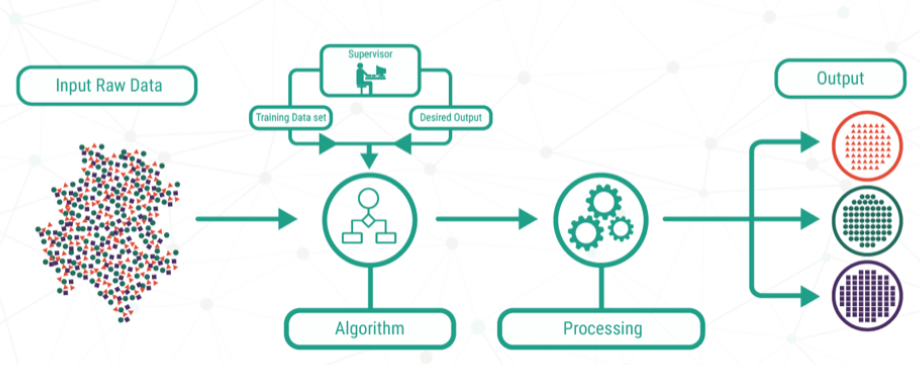
\includegraphics[scale=0.8]{images/Chapter2/supervised-learning-2.PNG}
% \caption{Example of Supervised Learning \cite{sup_unsup_learning}}
% \label{ex-sl}
% \end{figure}
% \par
% For example, there is a system that has to detect whether an email is a spam or not. We have two categories for the classification: "Spam" and "Not-spam". Classification can be multiple as well. So, in the beginning, we are feeding the examples of both spam emails and not-spam(normal) emails to our model. The given examples or dataset to the system are properly labeled with its right class. Here, it is important to note that we have to feed the system enough examples in different formats or templates so that it can generalize the data well. After passing the data to the system, it processes the input and stores the rules and features for each classification class. After the model training, it will return the system which can predict future emails as spam or not spam. This thesis problem also aims to use supervised learning methodology to classify the tax-related document. 
% \newline
% \newline
% Furthermore, supervised learning is further classified into two categories which are \textbf{Regression} and \textbf{Classification}
% \begin{enumerate}[label=(\alph*)]
%     \item \textbf{Regression:}
%     \par
%     In supervised learning, regression algorithms are used to estimate a mapping function (f) from the input variable (x) to continuous output variables (y). In simpler words, the output will always be in the form of continuous values means numbers. This continuous value can be either integer or float. It is mostly used to predict the amount or quantity. For example, by providing the KPIs of a company for the past 20 years we can use a regression algorithm to predict the KPI for next year.
%     \item \textbf{Classification:}
%     \par
%     On the other hand, classification is used to predict or map the category of the given input instead of a value. The result of the classification algorithm will always be in the form of a discrete value. We normally use this methodology to assign classes to the given datasets. Since our thesis problem is related to the classification problem, we can take our problem to give an example. For example, given multiple tax-related documents to the classification algorithm, it will classify or predict the class/type of the document for the given dataset. Classification also has multiple types. For instance, if the classification is being done for only two classes then it is called \textbf{Binary Classification}. However, if we are dealing with more than two classes and the model has to predict a single class for a dataset from multiple classes then this problem is called \textbf{Multi-class} classification. Another type is where the model has to predict data into multiple classes with percentage then this is called \textbf{Multi-Label Multi-class} Classification.
% \end{enumerate}
% \subsection{Unsupervised Learning}
% \par
% In unsupervised learning, as the name suggests there is no supervision or help provided about the dataset to the model. In this scenario, we do not know the result of the prediction or classification. Here, we pass plain and unstructured data to the model and now it's the job of the model to detect and recognize the pattern from the dataset and learn from it. It is normally used to extract the insights from the unstructured data and to cluster the data into multiple groups without knowing the actual categories.
% \begin{figure}[H]
% \centering
% 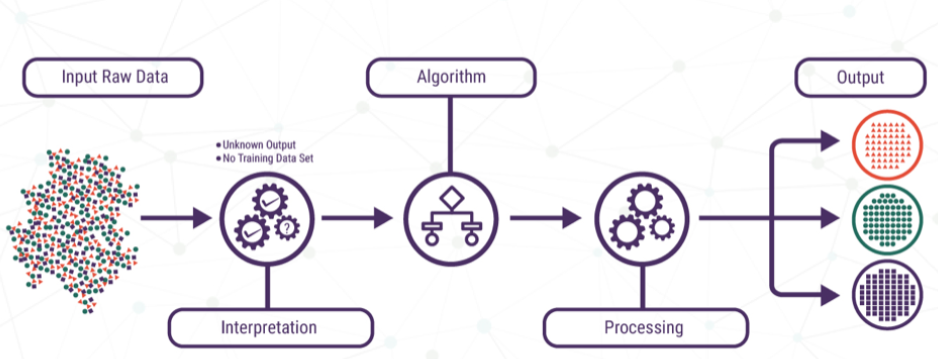
\includegraphics[scale=0.7]{images/Chapter2/unsupervised-learning.PNG}
% \caption{Example of Unsupervised Learning \cite{sup_unsup_learning}}
% \label{ex-ul}
% \end{figure}
% \par
% As you can see in the Figure \ref{ex-ul}, we are providing raw data to the model which means there is no label attached to the dataset, it is a totally new dataset for the model, and it does not have any knowledge about the types. Here what will the model do is to start looking for the pattern in the dataset. For instance, if the dataset is in the form of text and the model is getting particular keywords in some of the data every time then it will cluster these datasets into a different group and at the end, it will cluster all the data into different groups based on its finding.
% \subsection{Reinforcement Learning}
% \par
% Reinforcement learning is a methodology where the model learns over time by interacting with the environment. We can consider it as an intelligent system that learns from its experiences. For example, if the system is exposed to an environment and it has to predict the class of an image, it may happen that it will predict the wrong class but what will happen at that point is that someone will correct the system and tell the model about the correct class. Here, the model will update its information and will try to predict it correctly next time based on its previous experience. So, in reinforcement learning, the model is in continuous contact with the agents who correct the system about the wrong prediction and ultimately it will get mature by time and start predicting correctly.
% \begin{figure}[H]
% \centering
% 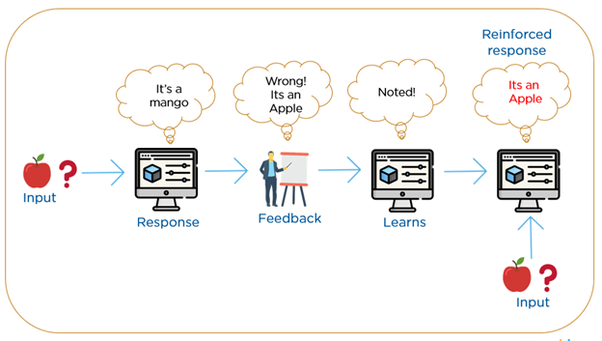
\includegraphics[scale=0.7]{images/Chapter2/reinforcement-learning.png}
% \caption{Example of Reinforcement Learning \cite{rei_learning}}
% \label{ex-rl}
% \end{figure}
% \section{Artificial Neural Network}
% Historically, neural networks are responsible for the revival of interest in machine learning. The subject of Artificial Neural Network (ANN) has matured to a great extent over the past few years and especially with the advent of very high-performance computing, the subject has assumed a tremendous significance and has got a very big application potential in very recent years. It met a lot of success in practical applications and got people going. Furthermore, many organizations are using it as a standard for example in banking and credit approval, medicine study, disease diagnosis neural networks are often used.
% \section{Definition and Description}
% \q{Artificial Neural Network (ANN) is a computational model that takes the inspiration of how the human brain works and how it processes the information and tends to replicate it as a system. In this system, it learns to perform tasks by learning from past examples without being programmed.} \cite{ann_def}
% \newline
% \newline
% \par
% Artificial Neural Network also known as Neural Network is part of a broader family of machine learning. This computational model is used to make intelligent systems. ANN basically mimics the way the human brain works and is also built on the same pattern. For example, if we want to teach a program to do a specific task then what are the possibilities of teaching that we can think of? The very basic approach is to write the whole program in the form of instructions (programming code) where the program will follow the instructions and perform the task accordingly. This program is not intelligent and is totally dependent on the given instruction. On the other hand, we can let the program to learn on its own which means we can apply artificial intelligence in the form of neural networks. 
% \par
% As I mentioned earlier, neural networks are capable of performing a task the way human beings do but in case of human beings they are not explicitly programmed instead a human mind learns themselves from examples and experiences and next time when it has to perform the same task, it follows the previous learning from examples and performs the tasks. For instance, let's take the example of our thesis problem where we have to classify the tax-related documents. If we ask a human being to classify and recognize these tax documents, then how a human brain will perform it? Well, it depends, if there is a document that a human brain never saw or processed before then obviously it will not recognize it at first because there is no previous learning or example that exists related to this document. In this case, the human brain will store this experience. Obviously, one example is not sufficient to generate a concrete memory and the human brain has to go through several documents of the same type to finally generate reliable learning and memory. When the human brain was going through these documents, what happened is that it analyzes the document, detects the patterns or keywords. Let say, in case of a salary slip document, there are many keywords that are always present normally such as net income, gross income, income tax, insurance tax, etc. So, what human brain will do is to store these keywords or if the document pattern or structure is the same then it also stores it as a feature. Now, next time when it has to recognize the same document, it will look for the same keywords and patterns which it has seen in the previous examples and made a decision based on that whether a document is of which type. This is a small example of human brain capacity and methodology to perform any task.  In the same way, the neural network learns from the examples given to it, develop the rules by processing, extracting and storing the features in different ways and use this learning to perform future tasks related to it.

% \section{Architecture of Neural Network}
% The basic architecture of a neural network consists of three layers: input, hidden layer and output. However, these hidden layers can be increased as well within a neural network. Each layer consists of neurons that are fully connected with each other. These connections are responsible to transmit data from one neuron to another. Below Figure \ref{ann-archi} is an example of a basic neural network architecture.
% \begin{figure}[H]
% \centering
% 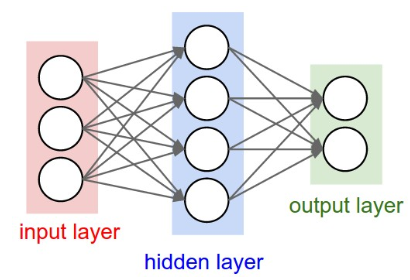
\includegraphics[scale=0.7]{images/Chapter2/ann-arch.PNG}
% \caption{Architecture of Neural Network \cite{ann_arch}}
% \label{ann-archi}
% \end{figure}
% \par
% As we see that neural network built on a layered architecture and each layer consist of neurons and are responsible for a particular job. Here the input layer is responsible for receiving data from outside the network it means whenever we feed data to the neural network to learn something it first passed through the input layer. Some scientists have said that the neurons in the input layer are different from the neurons in the subsequent layers and they do not receive information from the previous layer. It also makes sense to an extent because this input layer is the entry point to the network and does not contain any previous layer. So, in simpler words, the input layer is only responsible to receive data from outside and pass it on to the subsequent layer which is a hidden layer to process the data. The hidden layer is found between the input and output layers. As I said, the hidden layer in neural networks contains a minimum of one layer and then the number of hidden layers can be increased or decreased based on the complexity of the problem. The primary role of is layer is to receive data from the input layer and do some processing on this data like feature extraction, storing the features in the form of edges, etc. and produce the output by an activation function for the next layer. In short, all the processes related to the learning of the neural network is performed in the layer. The output layer which is the final layer is responsible to receive the data from the hidden layer and ultimately produce the end-result for the neural network.
% \section{In-depth detail of Artificial Neural Network}
% In this section, we will dive deep into the world of neural networks and will see the internal processing of neural networks. In the previous section, we described the different layers involved in the network and what are the responsibilities of each layer. Each layer consists of interconnected neurons or also known as nodes. In artificial neural networks, artificial neurons built by taking inspiration from the biological neurons present in the human brain.
% \begin{figure}[H]
% \centering
% 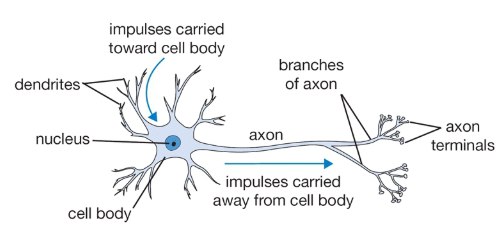
\includegraphics[scale=0.9]{images/Chapter2/neuron.PNG}
% \caption{Illustration of Biological Neuron \cite{ann_arch}}
% \label{neuron}
% \end{figure}
% \par
% In a biological neuron, \q{Dendrites} are responsible to receive the chemical signals from other neurons then applies a summation function which is adding all the inputs multiplies by the weight associated with it and then the \q{Axon} receives the output of summation and then passed it to the other neurons as a signal. An artificial neuron, somewhat, behaves in the same way as the biological neuron does. Likewise, artificial neurons in the neural network are the most fundamental computational unit which takes input from the different neurons, then applies some function to generate an output which is later on passed to some other neuron. Each input received by the neuron has a weight "w" associated with it and in the function, we take the summation of input x multiplied by its weight to generate the output Y. Below is the picture representing the described process.
% \begin{figure}[H]
% \centering
% 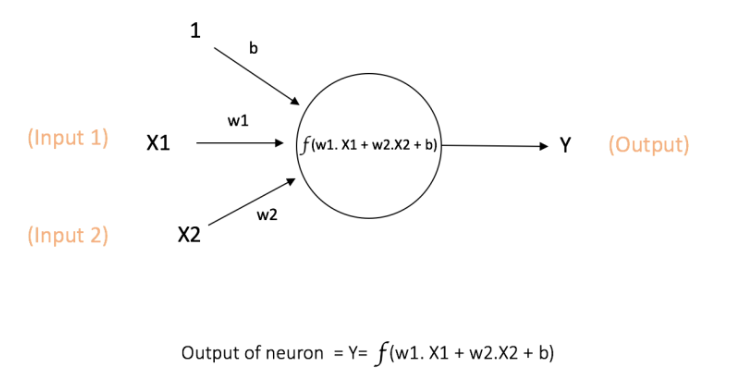
\includegraphics[scale=0.9]{images/Chapter2/neuron-summation-func.png}
% \caption{Artificial Neuron \cite{intro_to_nn}}
% \label{neuron-sum-func}
% \end{figure}
% \par
% In general, whenever a neural network is used to solve a problem, we first train our neural network by feeding the data to it. This data entered through the input layers and then pass it on to the hidden layers which are basically responsible for analyzing the data learn from it. If the hidden layers are multiple then in each layer, it stores different types of information. The result of the hidden layer(s) is the final output which is passed on to the output layer and then can be consumed by the system. Let's understand it with the help of below example of how neural network learns from the data.
% \begin{figure}[H]
% \centering
% 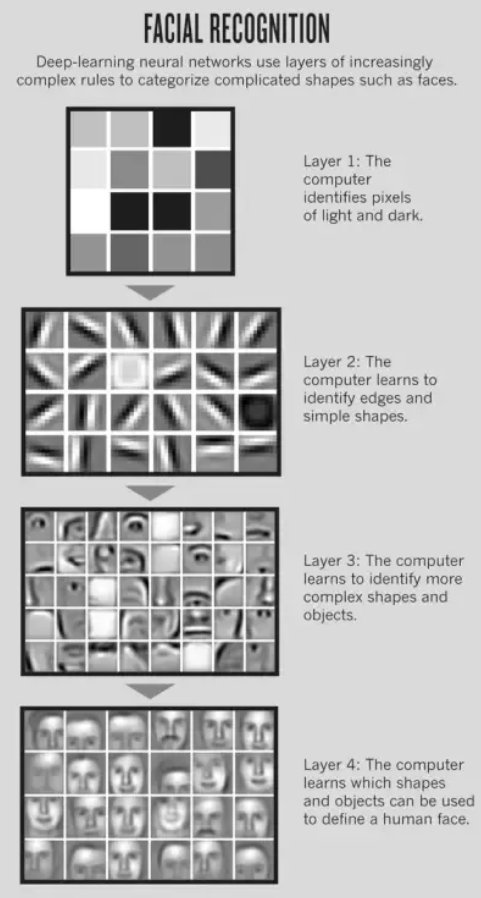
\includegraphics[scale=0.6]{images/Chapter2/ANN-example.PNG}
% \caption{Facial recognition example of Neural Network \cite{hidden_layer}}
% \label{fr-ex-neural-network}
% \end{figure}
% \par
% In the above example, the task is to detect a human face with the help of a neural network. For this, they are using a neural network that consists of multiple hidden layers and in the above diagram, these layers can be considered as the hidden layers. As you can see, each layer is storing some kind of information that is used to identify any particular information and the complexity of information is increasing by each layer. The first layer is used to identify the pixels of data then in the second layer, it identifies the edges from the data by the help of information from the first layer. In the third layer, it broke down the information into different human face objects like nose, ears, eyes mouth, etc. and trying to identify them. By the fourth layer, the network can detect a human face.
% \section{Convolutional Neural Network (CNN or ConvNet)}
% Convolutional Neural Network (CNN) is a type of artificial neural network which consists of convolutional layers and has been very successful particularly related to computer vision tasks such as recognizing objects, scenes, faces, etc. among many other applications. We have probably seen them in action anywhere a computer is identifying objects in an image, but we can also use the convolutional neural network in natural language procession projects which are primarily used for text classification too. The fact that they are useful for these fast-growing areas is one of the reasons they are so important in deep learning and artificial intelligence domain today. Once we understand how CNN works and what makes it unique from other neural networks, we can see why they are so effective for processing and classifying images.
% \newline
% \par
% But let's first take a regular neural network. A regular neural network has an input layer, hidden layers, and an output layer. The input layer accepts input in different forms while the hidden layers are responsible for performing calculations on these inputs and the output layer then delivers the outcome of the calculations and extractions. Each of these layers contains artificial neurons that are connected to neurons in the previous layer and each neuron has its own weight. This means we are not making any assumptions about the data being fed into the network. Usually, it works but not if you are working with images or a language. CNN works differently as they treat data as spatial. Instead of neurons being connected to every neuron in the previous layer, they are instead only connected to neurons close to it and all have the same weight. This simplification in the connection means the network upholds the spatial aspect of the dataset. The word convolutional refers to the filtering process that happens in this type of network. Think of it this way, an image is complex, and a convolutional neural network simplifies so it can better be processed and understood.
% \section{Architecture of Convolutional Neural Network}
% \begin{figure}[H]
% \centering
% 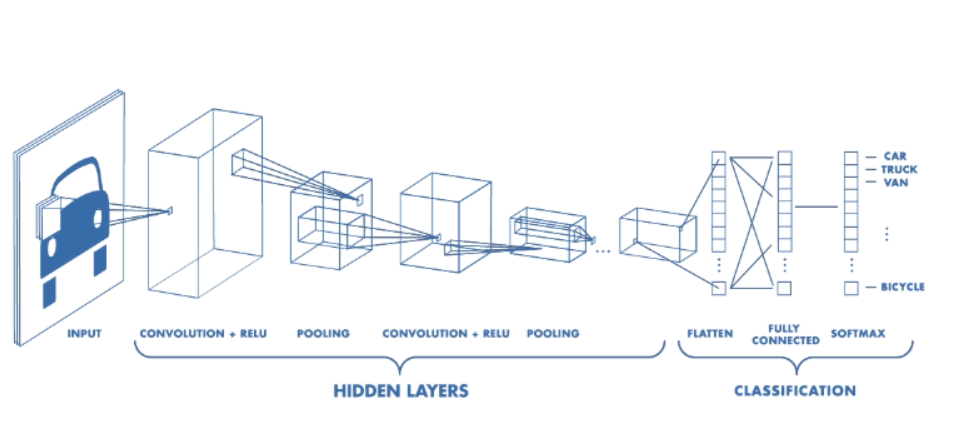
\includegraphics[scale=0.7]{images/Chapter2/cnn-arch.png}
% \caption{Architecture of Convolutional Neural Network \cite{arch_cnn}}
% \label{cnn-arch}
% \end{figure}
% \par
% Let's look at what is inside a convolutional neural network architecture. Like a normal neural network, a CNN is made up of multiple layers. There are a couple of layers that make it unique which are the \q{convolutional layer} and the \q{pooling layer}. However, like other neural networks, it will also have an \q{activation function} and a fully connected layer. The activation function layer ensures the non-linearity as the data moves through each layer in the network. Without it, the data being fed into each layer would lose the dimensionality that we want to maintain. On the other hand, the fully connected layer meanwhile allows us to perform classification on the dataset. In this architecture, the convolutional layer is the most important layer. It works by placing a filter over an array of image pixels and this then creates what is called a convolved feature map. It's a bit like looking at an image through a window which allows you to see specific features you might not otherwise be able to see. Next, we have the pooling layer. Its firsts reduce the sample size of a particular feature map. This also makes processing much faster as it reduces the number of parameters the network needs to process. The output of this is a pooled feature map. There are two ways of doing this, \q{max pooling} which takes the maximum input of a particular convolved feature or \q{average pooling} which simply takes the average. These steps are used for feature extraction whereby the network builds up a picture of the image data. If we want to perform classification, you will need to move into the fully connected layer. To do this, we will need to \q{flatten} things out. Remember, a neural network with a more complex set of connections can only process linear data.
% \newline
% \par
% Throughout the years, several scientists have worked and proposed different architectures of CNN. Few of them are \textbf{LeNet}(1990s), \textbf{AlexNet}(2012), \textbf{ZF Net}(2013), \textbf{GoogleNet}(2014), \textbf{VGGNet}(2014), \textbf{ResNet}(2015), etc. In this thesis, we have used the VGGNet architecture of CNN to classify the tax-related documents.
% \section{Operations in Convolutional Neural Network}
% There are couple of operations involved for different purposes within the convolutional neural network. Here, we will have a look on them one by one.
% \subsection{Activation Function}
% In CNN, the Activation function \cite{activation_func} is used to introduce non-linearity in the output of the neuron. When neuron generates the output by the weighted sum of inputs and adding bias then activation function is responsible to decide whether this output should be considered as fired neuron not to the other neurons. Some of the common activation functions are ReLU, Sigmoid, Softmax, tanh, etc.
% \subsection{Convolution}
% In a convolutional neural network architecture, we use a convolution operation in the convolutional layer. The main goal of the convolution operation is to maintain the spatial connection between pixels. It works by placing a filter over an array of image pixels and this then creates what is called a convolved feature map.
% \subsection{Bath Normalization}
% Batch normalization is the process of implementing normalization to the activation layer by subtracting the batch mean and dividing by the batch standard deviation. The main purpose of doing so it to faster the process of training within the convolutional neural network.
% \subsection{Pooling}
% The pooling operation is used to reduce the dimensionality of the feature maps, but it retains the most important information. The output of this operation is called Pooled Feature Map. There are two types of pooling, \textbf{max pooling} that takes the largest element from the feature map within a window and the \textbf{average pooling} which takes the average of all the elements within a window.
% \subsection{Padding}
% Padding operation is used to add more window to the image by adding extra pixels at the border of the image. It is used to retain a better understanding of the edges of the image by centralizing it. Some of the padding's operations are \textbf{zero padding} and \textbf{reflection padding}. 

\section{Neural Network}
Neurons and nodes connected with each other is neural network. These neurons are modeled as human brain neurons. Neural network is artificially created network which can work like human brain. Connected between neurons are represented by weights of neurons. Let us study biological neuron to get how neurons of artificial neural network works.
\par
Human brain is the most completed neural network which consists of trillions of neurons and have billions of connections with each other. Electrical signals are used to do communication between biological neurons. Figure \ref{neuron} shows the structure of biological neuron.
\begin{figure}[H]
  \centering
  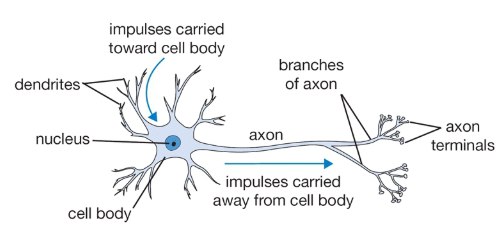
\includegraphics[scale=0.14]{images/Chapter2/neuron.png}
  \caption{Structure of Neuron \cite{neuron}}
  \label{neuron}
\end{figure}
\par
The output is determined by \textit{Cell Body} of neuron. \textit{Axon} is output from neuron and \textit{Dendrites} are input to neuron.

\subsection{Artificial Neural Network}
Similar behavior as biological neuron can be achieved by create neuron using programming. Every neuron is connected to more than one neuron and takes input from connected neurons. By using mathematical computation with weight and input, neuron gives an output. This output is passed to outgoing neurons.
\par
Neurons are connected very strongly with each other and are in different layers. First layer represents input and last layer represents output. The layers in between are known as hidden layer. Figure \ref{fig:ann} shows an artificial neural network having 3 neurons in input layer, 2 neurons in output layer, and 5 neurons in hidden layer.

\begin{figure}[H]
  \centering
  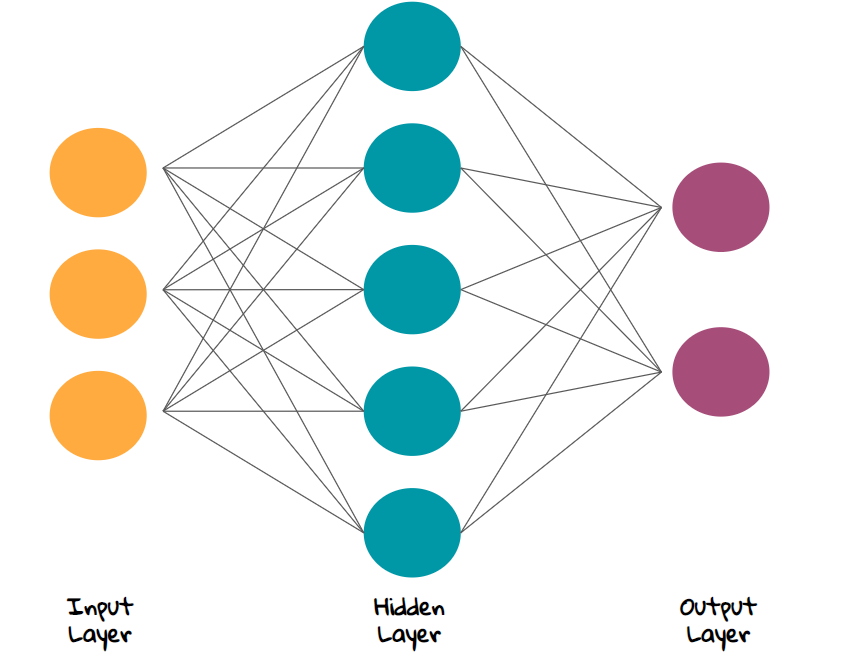
\includegraphics[scale=0.45]{images/Chapter2/ann.png}
  \caption{Architecture of Artificial Neural Network \cite{fig_ann}}
  \label{fig:ann}
\end{figure}

\section{Convolutional Neural Network}
Convolutional Neural Network (CNN) is category of deep learning algorithm which is used to distinguish object from each other. A deep neural network is an artificial neural network (ANN) with multiple hidden layers between the input and output layers. CNN are also known as ConvNet. \q{Convolutional networks are at the core of most state of-the-art computer vision solutions for a wide variety of tasks} \cite{Szegedy_2016_CVPR}. Convolutional neural networks has become the go to network for computer vision tasks such as object detection, image classification and semantic segmentation. It also need very less preprocessing in comparision with other classifiers.
\begin{figure}[H]
  \centering
  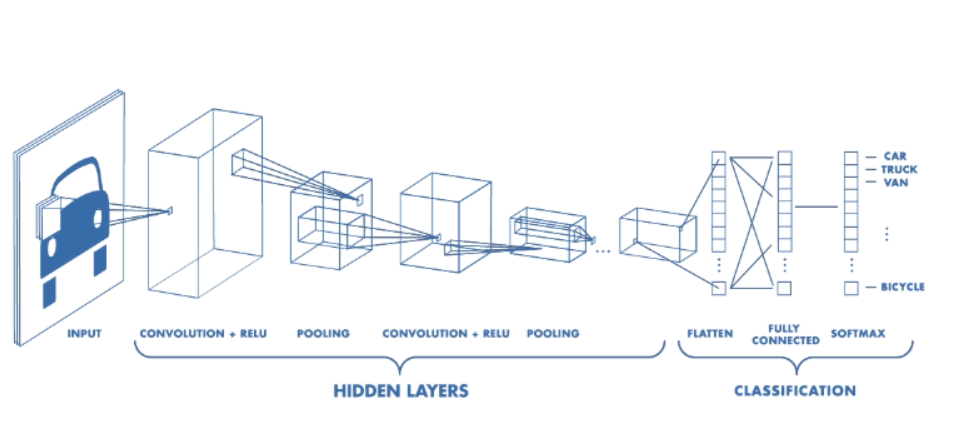
\includegraphics[scale=0.7]{images/Chapter2/cnn-arch.png}
  \caption{Convolutional Neural Network \cite{arch_cnn}}
  \label{cnn-arch}
\end{figure}
\subsection{Architecture of Convolutional Neural Network}
CNN takes image as an input and gives classification or regression score as an output. Image is given to CNN as a first layer and classification or regression score as output layer. The layers in-between input layer and output layers are hidden layers. The number of hidden layers depends on the problem statement. There are many different types of hidden layers with different purposes. There could be convolutional layer, pooling layer, and ReLU layer. Figure 1 \ref{cnn} shows a simple CNN.
\begin{figure}[H]
  \centering
  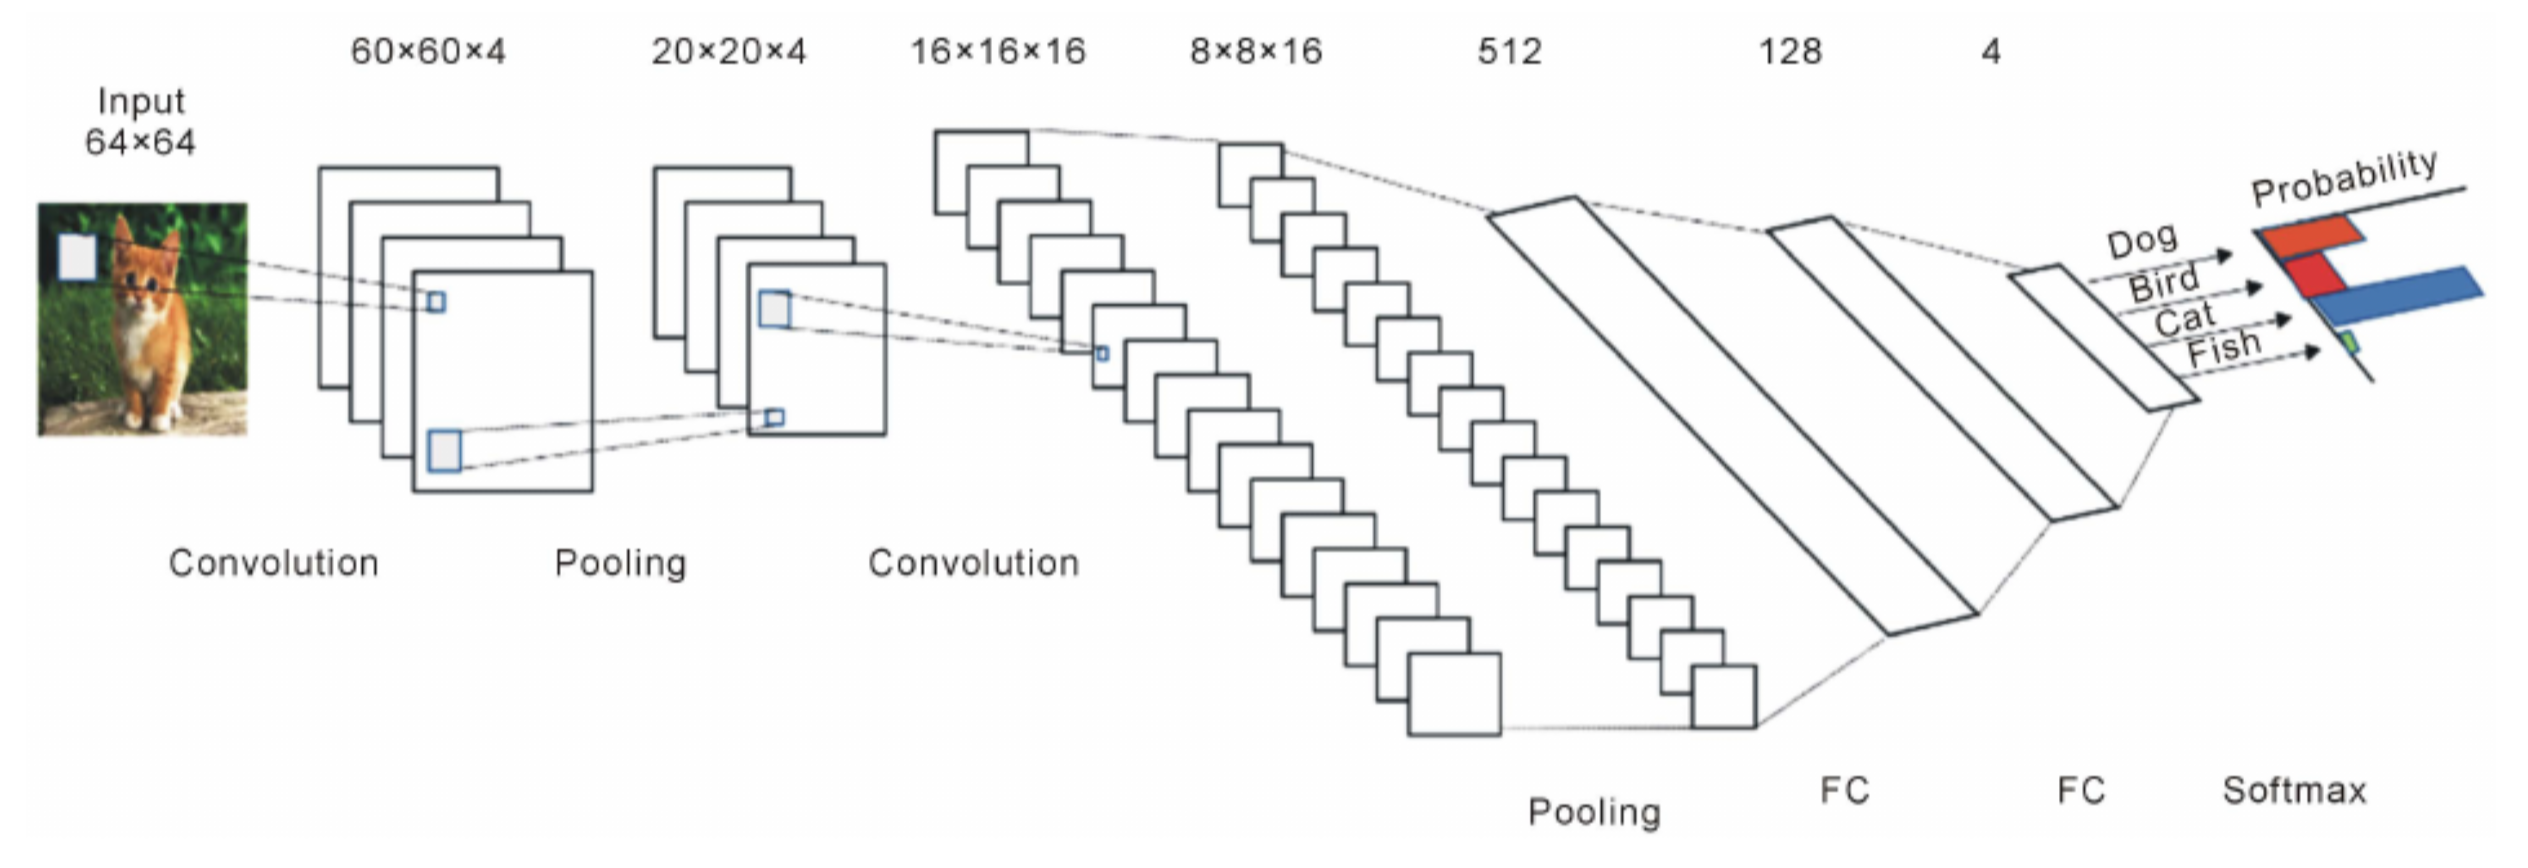
\includegraphics[scale=0.35]{images/Chapter2/cnn.png}
  \caption{Architecture of Convolutional Neural Network \cite{cnn_arch_image}}
  \label{cnn}
\end{figure}

Following are the operations performed in CNN:

\begin{itemize}
  \item \textbf{Convolution: } The main purpose of convolutional layer is to extract features from an image. Features could be corners, shape type, edges, contrast, etc. Different features are extracted by applying different filters. Convolution is done in convolutional layers. Example of convolution operation performed on an image are shown in Figure \ref{convolution}. 
  \begin{figure}[H]
    \centering
    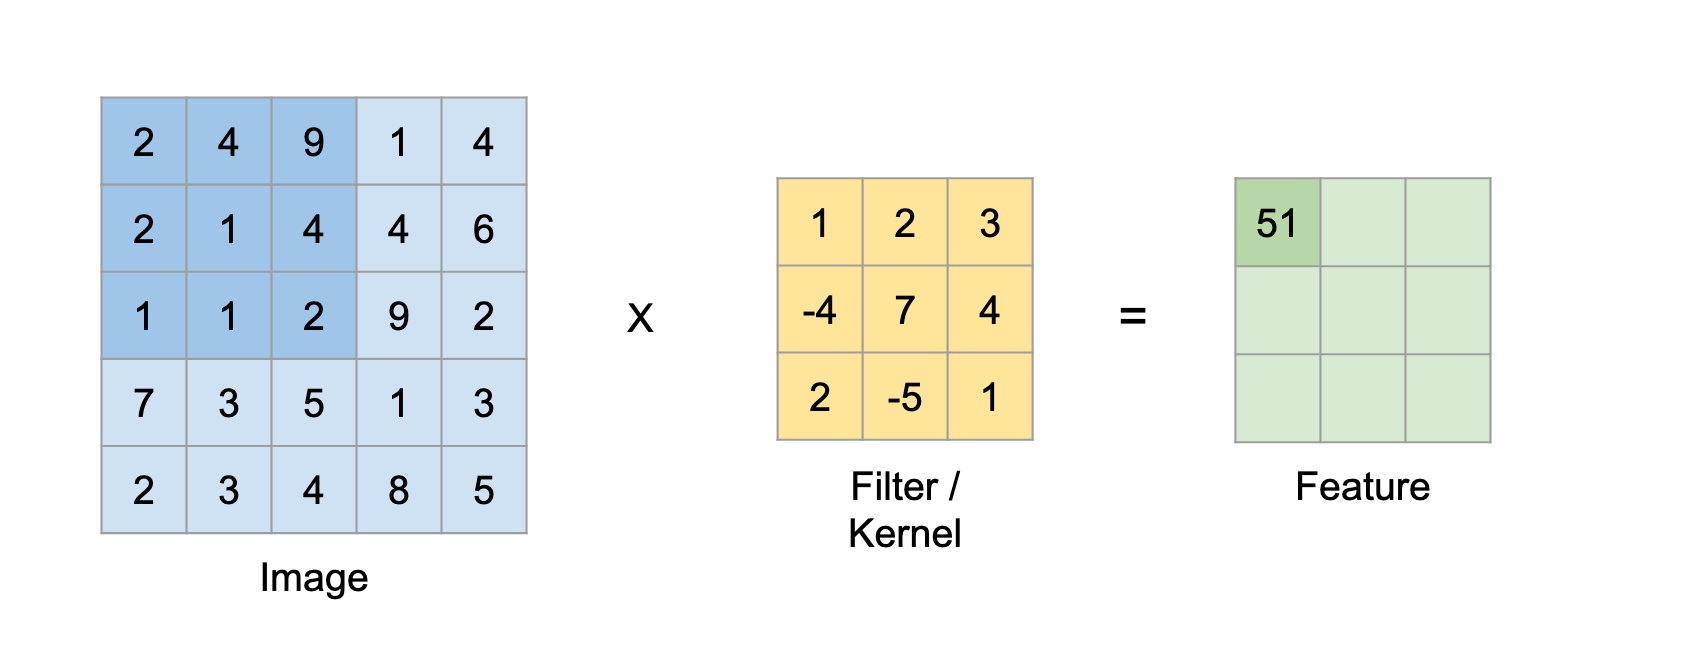
\includegraphics[scale=0.25]{images/Chapter2/convolution.png}
    \caption{Architecture of Convolutional Neural Network \cite{conv}}
    \label{convolution}
  \end{figure}
  Filter of dimensions with 3 x 3 is placed on second row, second column of image. The convolution operation is done by doing dot product between filter and the patch of image. This patch is shown in dark blue color to differentiate it. Dot product is taken by doing element-wise multiplication and sum it. The answer of it is saved in Feature. Filters having different values extract different types of features from images. These features are called as feature maps.
  \item \textbf{Padding: } The main purpose of padding is to preserve the dimension. As it can be seen in Figure 2, that after doing convolution the dimensions of input got reduced from 5 x 5 to 3 x 3. The reduction in dimension was not required here and it also causes problems in architecture design as it was not necessary. Padding is done to remove this problem. Zero padding is the most used padding technique. Row or column of zeros are appended with the start and end of image to increase the dimensions of image. The dimensions of image are increased in such a way that the dimensions of the result after doing convolution remains the same as the original image.
  \item \textbf{ReLU: } The result of the convolution is passed from ReLU (Rectified Linear Unit) function layer. The main purpose of this layer is to add non-linearity into process. Non-linearity can be added by using different functions e.g. Sigmoid, Tahn etc. Than and Sigmoid are very computational expensive. ReLU was introduced to include non-linearity. It is not computational expensive and is very easy to do. The results of CNN using Than, Sigmoid on other hand CNN using ReLU were same. So, researchers started using ReLU as Non-linearity layer. ReLU function converts negative values to Zero and does not change non-negative values. Graphical representation of ReLU function is shown in Figure \ref{relu}.
  \begin{figure}[H]
    \centering
    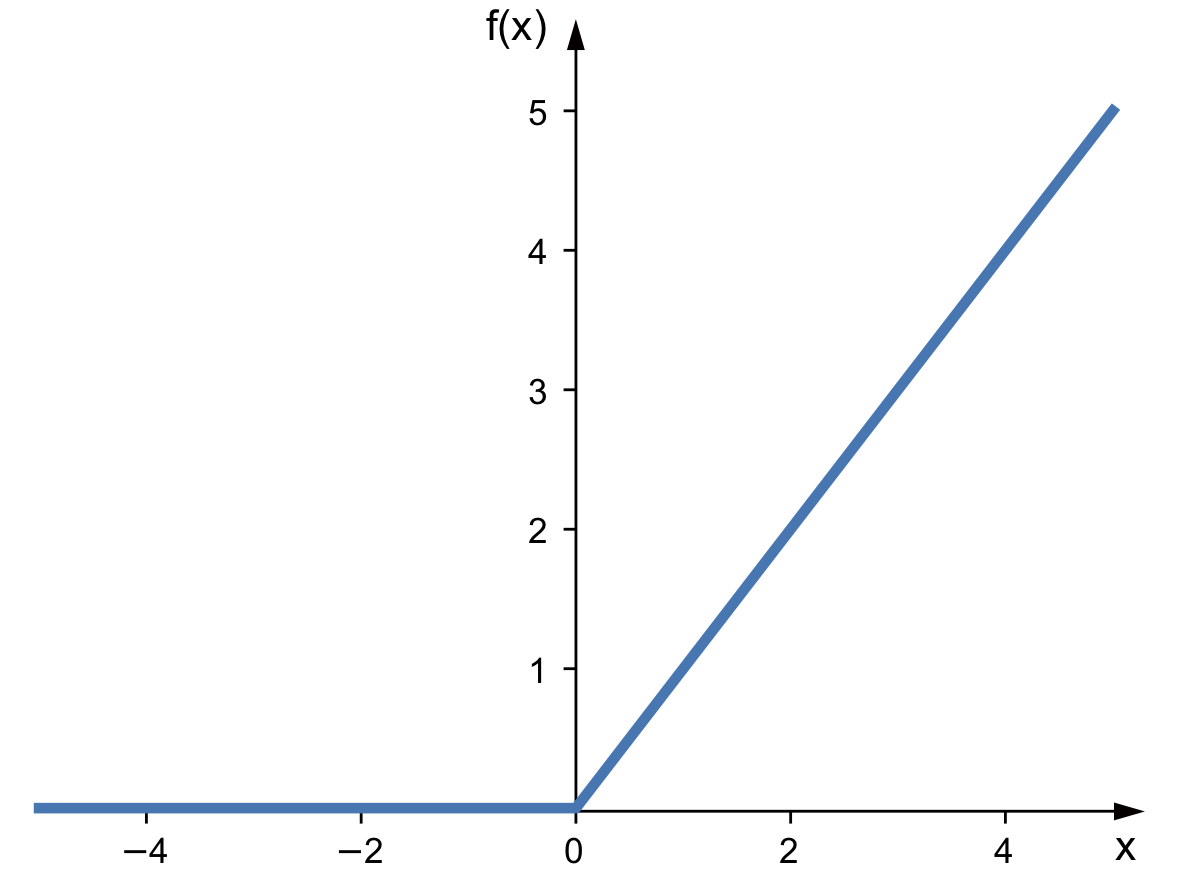
\includegraphics[scale=0.7]{images/Chapter2/relu.png}
    \caption{Rectified Linear Unit \cite{relu}}
    \label{relu}
  \end{figure}
  \item \textbf{Pooling: } Pooling is done after doing ReLU. Down sampling is done by using pooling. The purpose of reducing the dimensions is to reduce the number of parameters. Sum, mean and max pooling are popular image processing techniques. As the name says, taking maximum out of a patch of image is max-pooling. Max-pooling filter of dimensions 2 x 2 with a stride of 2 reduces the dimensions into half. Example of it is shown in Figure 4.
  \begin{figure}[H]
    \centering
    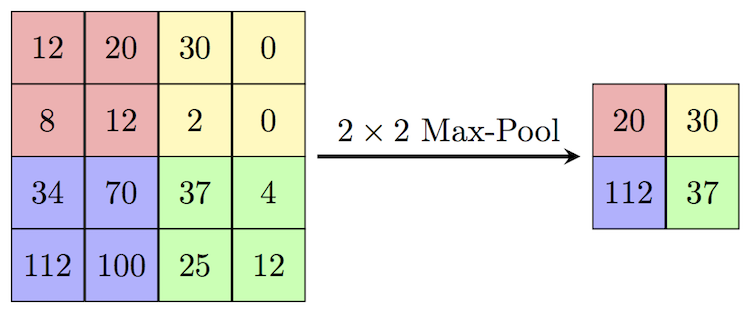
\includegraphics[scale=1.0]{images/Chapter2/pooling.png}
    \caption{Pooling \cite{pooling}}
    \label{pooling}
  \end{figure}
  \item \textbf{Fully Connected Layer: } Classification is done in fully connected layers (FC layers). As convolutional layers are responsible for extracting features, fully connected layers are responsible for classification. Output of fully connected layers can be a matrix for multi-class classification or a single value for regression.
\end{itemize}
